\subsection{CARTAN SUBALGEBRAS}

DEFINITION 1. Let \(\mathfrak{g}\) be a Lie algebra. A Cartan subalgebra of \(\mathfrak{g}\) is a nilpotent subalgebra of \(\mathfrak{g}\) equal to its own normalizer.

Later we shall obtain the following results:

\begin{enumerate}
\def\labelenumi{\arabic{enumi})}
\item
  if \(k\) is infinite, \(\mathfrak{g}\) has Cartan subalgebras (no. 3, Cor. 1 of Th. 1);
\item
  if \(k\) is of characteristic zero, all Cartan subalgebras of \(\mathfrak{g}\) have the same dimension (§3, no. 3, Th. 2);
\item
  if \(k\) is algebraically closed and of characteristic 0, all Cartan subalgebras of \(\mathfrak{g}\) are conjugate under the group of elementary automorphisms of \(\mathfrak{g}\) (§3, no. 2, Th. 1).
\end{enumerate}

Examples. 1) If \(\mathfrak{g}\) is nilpotent, the only Cartan subalgebra of \(\mathfrak{g}\) is \(\mathfrak{g}\) itself (Chap. I, §4, no. 1, Prop. 3).

\begin{enumerate}
\def\labelenumi{\arabic{enumi})}
\setcounter{enumi}{1}
\item
  Let \(\mathfrak{g} = \mathfrak{gl}(n,k)\) , and let \(\mathfrak{h}\) be the set of diagonal matrices belonging to \(\mathfrak{g}\) . We show that \(\mathfrak{h}\) is a Cartan subalgebra of \(\mathfrak{g}\) . First, \(\mathfrak{h}\) is commutative, hence nilpotent. Let \((E_{ij})\) be the canonical basis of \(\mathfrak{gl}(n,k)\) , and let \(x = \sum \mu_{ij}E_{ij}\) be an element of the normalizer of \(\mathfrak{h}\) in \(\mathfrak{g}\) . If \(i\neq j\) , formulas (5) of Chap. I, §1, no. 2 show that the coefficient of \(E_{ij}\) in \([E_{ii},x]\) is \(\mu_{ij}\) . Since \(E_{ii}\in \mathfrak{h}\) , \([E_{ii},x]\in \mathfrak{h}\) , and the coefficient in question is zero. Thus \(\mu_{ij} = 0\) for \(i\neq j\) , so \(x\in \mathfrak{h}\) , which shows that \(\mathfrak{h}\) is indeed a Cartan subalgebra of \(\mathfrak{g}\) .
\item
  Let \(\mathfrak{h}\) be a Cartan subalgebra of \(\mathfrak{g}\) and let \(\mathfrak{g}_1\) be a subalgebra of \(\mathfrak{g}\) containing \(\mathfrak{h}\) . Then \(\mathfrak{h}\) is a Cartan subalgebra of \(\mathfrak{g}_1\) ; this follows immediately from Def. 1.
\end{enumerate}

PROPOSITION 1. Let \(\mathfrak{g}\) be a Lie algebra and let \(\mathfrak{h}\) be a Cartan subalgebra of \(\mathfrak{g}\) . Then \(\mathfrak{h}\) is a maximal nilpotent subalgebra of \(\mathfrak{g}\) .

Let \(\mathfrak{h}'\) be a nilpotent subalgebra of \(\mathfrak{g}\) containing \(\mathfrak{h}\) . Then \(\mathfrak{h}\) is a Cartan subalgebra of \(\mathfrak{h}'\) (Example 3), so \(\mathfrak{h} = \mathfrak{h}'\) (Example 1).

There exist maximal nilpotent subalgebras that are not Cartan subalgebras (Exerc. 2).

\pandocbounded{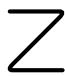
\includegraphics[keepaspectratio]{images/part001_35e3d035.jpg}}

PROPOSITION 2. Let \((\mathfrak{g}_i)_{i\in \mathrm{I}}\) be a finite family of Lie algebras and \(\mathfrak{g} = \prod_{i\in \mathrm{I}}\mathfrak{g}_i\)

The Cartan subalgebras of \(\mathfrak{g}\) are the subalgebras of the form \(\prod_{i\in I}\mathfrak{h}_i\) , where \(\mathfrak{h}_i\) is a Cartan subalgebra of \(\mathfrak{g}_i\) .

If \(h_{i}\) is a subalgebra of \(g_{i}\) with normalizer \(n_{i}\) , then \(\prod h_{i}\) is a subalgebra of g with normalizer \(\prod n_{i}\) ; if the \(h_{i}\) are nilpotent, \(\prod h_{i}\) is nilpotent; thus, if \(h_{i}\) is a Cartan subalgebra of \(g_{i}\) for all i, \(\prod h_{i}\) is a Cartan subalgebra of g. Conversely, let h be a Cartan subalgebra of g; the projection \(h_{i}\) of h onto \(g_{i}\) is a nilpotent subalgebra of \(g_{i}\) , and \(\prod h_{i}\) is a nilpotent subalgebra of g containing h; hence \(h = \prod h_{i}\) (Prop. 1); thus, for all i, \(h_{i}\) is its own normalizer in \(g_{i}\) , and so is a Cartan subalgebra of \(g_{i}\) .

Example 4. If k is of characteristic 0, \(\mathfrak{gl}(n,k)\) is the product of the ideals \(\mathfrak{sl}(n,k)\) and k.1. It follows from Example 2 and Prop. 2 that the set of diagonal matrices of trace 0 in \(\mathfrak{sl}(n,k)\) is a Cartan subalgebra of \(\mathfrak{sl}(n,k)\) .

PROPOSITION 3. Let g be a Lie algebra, h a subalgebra of g, and \(k'\) an extension of k. Then h is a Cartan subalgebra of g if and only if \(h \otimes_{k} k'\) is a Cartan subalgebra of \(g \otimes_{k} k'\) .

Indeed, \(\mathfrak{h}\) is nilpotent if and only if \(\mathfrak{h} \otimes_k k'\) is (Chap. I, §4, no. 5). On the other hand, if \(\mathfrak{n}\) is the normalizer of \(\mathfrak{h}\) in \(\mathfrak{g}\) , the normalizer of \(\mathfrak{h} \otimes_k k'\) in \(\mathfrak{g} \otimes_k k'\) is \(\mathfrak{n} \otimes_k k'\) (Chap. I, §3, no. 8).

PROPOSITION 4. Let \(\mathfrak{g}\) be a Lie algebra, \(\mathfrak{h}\) a nilpotent subalgebra of \(\mathfrak{g}\) . Then \(\mathfrak{h}\) is a Cartan subalgebra of \(\mathfrak{g}\) if and only if \(\mathfrak{g}^0 (\mathfrak{h}) = \mathfrak{h}\) .

If \(\mathfrak{g}^0 (\mathfrak{h}) = \mathfrak{h}\) , \(\mathfrak{h}\) is its own normalizer (§1, Prop. 10 (i)), so \(\mathfrak{h}\) is a Cartan subalgebra of \(\mathfrak{g}\) . Assume that \(\mathfrak{g}^0 (\mathfrak{h})\neq \mathfrak{h}\) . Consider the representation of \(\mathfrak{h}\) on \(\mathfrak{g}^0 (\mathfrak{h}) / \mathfrak{h}\) obtained from the adjoint representation by passage to the quotient. By applying Engel's theorem (Chap. I, §4, no. 2, Th. 1), we see that there exists \(x\in \mathfrak{g}^0 (\mathfrak{h})\) such that \(x\notin \mathfrak{h}\) and \([\mathfrak{h},x]\subset \mathfrak{h}\) ; then \(x\) belongs to the normalizer of \(\mathfrak{h}\) in \(\mathfrak{g}\) , so \(\mathfrak{h}\) is not a Cartan subalgebra of \(\mathfrak{g}\) .

COROLLARY 1. Let \(\mathfrak{g}\) be a Lie algebra, \(\mathfrak{h}\) a Cartan subalgebra of \(\mathfrak{g}\) . If \(k\) is infinite, there exists \(x \in \mathfrak{h}\) such that \(\mathfrak{h} = \mathfrak{g}^0(x)\) .

Indeed, \(\mathfrak{h} = \mathfrak{g}^0 (\mathfrak{h})\) and we can apply Prop. 9 (ii) of §1.

COROLLARY 2. Let \(f: \mathfrak{g} \to \mathfrak{g}'\) be a surjective homomorphism of Lie algebras. If \(\mathfrak{h}\) is a Cartan subalgebra of \(\mathfrak{g}\) , \(f(\mathfrak{h})\) is a Cartan subalgebra of \(\mathfrak{g}'\) .

Indeed, \(f(\mathfrak{h})\) is a nilpotent subalgebra of \(\mathfrak{g}'\) . On the other hand, consider the representation \(x \mapsto \operatorname{ad} f(x)\) of \(\mathfrak{h}\) on \(\mathfrak{g}'\) . By Prop. 9 (iv) of §1, no. 3, \(f(\mathfrak{g}^0(\mathfrak{h})) = \mathfrak{g}'^0(\mathfrak{h})\) . Now \(\mathfrak{g}^0(\mathfrak{h}) = \mathfrak{h}\) , and on the other hand it is clear that \(\mathfrak{g}'^0(\mathfrak{h}) = \mathfrak{g}'^0(f(\mathfrak{h}))\) . Hence, \(f(\mathfrak{h}) = \mathfrak{g}'^0(f(\mathfrak{h}))\) and it suffices to apply Prop. 4.

COROLLARY 3. Let \(\mathfrak{h}\) be a Cartan subalgebra of a Lie algebra \(\mathfrak{g}\) , and let \(\mathcal{C}^n\mathfrak{g}\) ( \(n \geq 1\) ) be a term of the descending central series of \(\mathfrak{g}\) (Chap. I, §1, no. 5). Then \(\mathfrak{g} = \mathfrak{h} + \mathcal{C}^n\mathfrak{g}\) .

Indeed, Corollary 2 shows that the image of \(\mathfrak{h}\) in \(\mathfrak{g} / \mathcal{C}^n\mathfrak{g}\) is a Cartan subalgebra of \(\mathfrak{g} / \mathcal{C}^n\mathfrak{g}\) , hence is equal to \(\mathfrak{g} / \mathcal{C}^n\mathfrak{g}\) since \(\mathfrak{g} / \mathcal{C}^n\mathfrak{g}\) is nilpotent (Example 1).

COROLLARY 4. Let \(\mathfrak{g}\) be a Lie algebra, \(\mathfrak{h}\) a Cartan subalgebra of \(\mathfrak{g}\) , and \(\mathfrak{a}\) a subalgebra of \(\mathfrak{g}\) containing \(\mathfrak{h}\) .

\begin{enumerate}
\def\labelenumi{(\roman{enumi})}
\item
  \(\mathfrak{a}\) is equal to its own normalizer in \(\mathfrak{g}\) .
\item
  Assume that \(k = \mathbf{R}\) or \(\mathbf{C}\) ; let \(G\) be a Lie group with Lie algebra \(\mathfrak{g}\) , A the integral subgroup of \(G\) with Lie algebra \(\mathfrak{a}\) . Then \(A\) is a Lie subgroup of \(G\) , and it is the identity component of the normalizer of \(A\) in \(G\) .
\end{enumerate}

Let n be the normalizer of a in g. Since h is a Cartan subalgebra of n (Example 3), \(\{0\}\) is a Cartan subalgebra of n/a (Cor. 2), hence is equal to its normalizer in n/a; in other words, n = a. Assertion (ii) follows from (i) and Chap. III, §9, no. 4, Cor. of Prop. 11.

COROLLARY 5. Let g be a Lie algebra, E a subset of g. Let E operate on g by the adjoint representation. Then E is a Cartan subalgebra of g if and only if \(E = \mathfrak{g}^{0}(E)\) .

The condition is necessary (Prop. 4). Assume now that \(\mathrm{E} = \mathfrak{g}^0 (\mathrm{E})\) . By Prop. 2 (ii) of §1, no. 1, E is then a subalgebra of \(\mathfrak{g}\) . If \(x\in \mathrm{E}\) , \(\mathrm{ad}_{\mathrm{E}}x\) is nilpotent since \(\mathrm{E}\subset \mathfrak{g}^0 (\mathrm{E})\) ; hence the algebra E is nilpotent. But then E is a Cartan subalgebra by Prop. 4.

COROLLARY 6. Let g be a Lie algebra, let \(k_{0}\) be a subfield of k such that \([k:k_{0}]<+\infty\) , and let \(g_{0}\) be the Lie algebra obtained from g by restricting the field of scalars to \(k_{0}\) . Let h be a subset of g. Then h is a Cartan subalgebra of g if and only if h is a Cartan subalgebra of \(g_{0}\) .

This follows from Cor. 5, since the condition \(\mathfrak{h} = \mathfrak{g}^0 (\mathfrak{h})\) does not involve the base field.

PROPOSITION 5. Let g be a Lie algebra, c its centre, h a vector subspace of g. Then h is a Cartan subalgebra of g if and only if h contains c and h/c is a Cartan subalgebra of g/c.

Assume that \(\mathfrak{h}\) is a Cartan subalgebra of \(\mathfrak{g}\) . Since \([\mathfrak{c},\mathfrak{g}]\subset \mathfrak{h}\) , we have \(\mathfrak{c}\subset \mathfrak{h}\) . On the other hand, \(\mathfrak{h} / \mathfrak{c}\) is a Cartan subalgebra of \(\mathfrak{g} / \mathfrak{c}\) by Cor. 2 of Prop. 4.

Assume that \(\mathfrak{h} \supset \mathfrak{c}\) and that \(\mathfrak{h} / \mathfrak{c}\) is a Cartan subalgebra of \(\mathfrak{g} / \mathfrak{c}\) . Let \(f\) be the canonical morphism from \(\mathfrak{g}\) to \(\mathfrak{g} / \mathfrak{c}\) . The algebra \(\mathfrak{h}\) , which is a central extension of \(\mathfrak{h} / \mathfrak{c}\) , is nilpotent. Let \(\mathfrak{n}\) be the normalizer of \(\mathfrak{h}\) in \(\mathfrak{g}\) . If \(x \in \mathfrak{n}\) , \([f(x), \mathfrak{h} / \mathfrak{c}] \subset \mathfrak{h} / \mathfrak{c}\) , hence \(f(x) \in \mathfrak{h} / \mathfrak{c}\) , and so \(x \in \mathfrak{h}\) . This proves that \(\mathfrak{h}\) is a Cartan subalgebra of \(\mathfrak{g}\) .

COROLLARY. Let \(\mathcal{C}_{\infty}\mathfrak{g}\) be the union of the ascending central series of the Lie algebra \(\mathfrak{g}\) (Chap. I, §1, no. 6). The Cartan subalgebras of \(\mathfrak{g}\) are the inverse images of the Cartan subalgebras of \(\mathfrak{g}/\mathcal{C}_{\infty}\mathfrak{g}\) .

Indeed, the centre of \(\mathfrak{g} / \mathcal{C}_i\mathfrak{g}\) is \(\mathcal{C}_{i + 1}\mathfrak{g} / \mathcal{C}_i\mathfrak{g}\) , and the corollary follows immediately from Prop. 5 by induction.

Remark. \(C_{\infty}g\) is the smallest ideal n of g such that the centre of g/n is zero; it is a characteristic and nilpotent ideal of g.

